% XCircuit output "sna_meas.tex" for LaTeX input from sna_meas.ps
\def\putbox#1#2#3#4{\makebox[0in][l]{\makebox[#1][l]{}\raisebox{\baselineskip}[0in][0in]{\raisebox{#2}[0in][0in]{\scalebox{#3}{#4}}}}}
\def\rightbox#1{\makebox[0in][r]{#1}}
\def\centbox#1{\makebox[0in]{#1}}
\def\topbox#1{\raisebox{-0.60\baselineskip}[0in][0in]{#1}}
\def\midbox#1{\raisebox{-0.20\baselineskip}[0in][0in]{#1}}
   \scalebox{1}{
   \normalsize
   \parbox{4.58854in}{
   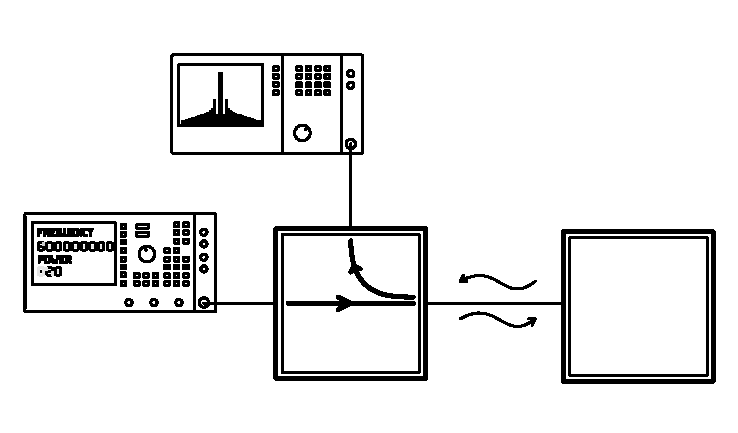
\includegraphics[scale=1]{sna_meas}\\
   % translate x=113 y=390 scale 0.38
   \putbox{3.19in}{0.42in}{1.20}{\centbox{Incident}}%
   \putbox{3.19in}{0.23in}{1.20}{\centbox{power $P_i$}}%
   \putbox{3.21in}{1.21in}{1.20}{\centbox{Reflected}}%
   \putbox{3.21in}{1.02in}{1.20}{\centbox{power $P_r$}}%
   \putbox{2.25in}{1.07in}{1.20}{$X~\mr{dB}$}%
   \putbox{2.25in}{1.52in}{1.20}{\midbox{$P_s=P_r-X$}}%
   \putbox{4.14in}{0.75in}{2.40}{\centbox{\midbox{DUT}}}%
   \putbox{0.71in}{1.42in}{1.20}{\centbox{RF generator}}%
   \putbox{1.69in}{2.48in}{1.20}{\centbox{Spectrum analyzer}}%
   \putbox{2.25in}{0.09in}{1.20}{\centbox{Directional coupler}}%
   } % close 'parbox'
   } % close 'scalebox'
   \vspace{-\baselineskip} % this is not necessary, but looks better
